%%%%%%%%%%%%%%%%%%%%%%%%%%%%%%%%%%%%%%%%%%%%%%%%%%%%%%%%%%%%
% Pedro Brandão's trial to get a template for thesis for students
% Used the upthesis from Fernando Silva (see upthesis).
% See also the packages file.
% 2014/07/07 First draft
% 2014/07/21 
%  pbrandao: added the list of listings (it should produce portuguese name if
%           babel is set to portuguese, see packages.tex). Changed usepackage of babel
%           to be before input packages.tex to allow test

%
%%%%%%%%%%%%%%%%%%%%%%%%%%%%%%%%%%%%%%%%%%%%%%%%%%%%%%%%%%%%


% makes all pages the height of the text on that page. No extra vertical space is added.
\raggedbottom 
% setting it to report will remove the blank pages before each chapter
\documentclass[11pt,a4paper,twoside]{book}


%%%%%%%%%%%%%%%%%%%%%%%%%%%%%%%%%%%%%%%%%%%%%%%%%%%%%%%%%%%%
%%%   Packages that need to be configured for the thesis
%%%%%%%%%%%%%%%%%%%%%%%%%%%%%%%%%%%%%%%%%%%%%%%%%%%%%%%%%%%%

% Language settings
% use UKenglish for UK or leave blank for US English
% it will also change the names for some of the chapters (list of tables, figures, content,
%\usepackage[UKenglish]{babel}
\usepackage[portuguese]{babel}

%%%%%%%%%%%%%%%%%%%%%%%%%%%%%%%%%%%%%%%%%%%%%%%%%%%%%%%%%%%%
%%%   Packages uses language definitions
% see file below for more packages and settings
%%%%%%%%%%%%%%%%%%%%%%%%%%%%%%%%%%%%%%%%%%%%%%%%%%%%%%%%%%%%
\usepackage{upthesis}

\usepackage[
%backref={section},
%pagebackref, % for getting references to the page where the citation is (in the biblio)
pdfpagelabels=false
]{hyperref}
\hypersetup{pdftitle={Titulo da tese}, %nao suporta acentos
   pdfkeywords ={palavras chave},
   pdfsubject = {assunto},
	bookmarksnumbered=true,
   pdfauthor ={Autor}, % see other options on manual (can be page) needs empty line on bibitem
   plainpages=false, 
   pdfborder={0 0 0},
   colorlinks,%colorlinks=false,
   breaklinks=true,
	%linktocpage= false, make page number, not text, be link on TOC, LOF and LOT 
	%hyperindex=true 	% Makes the page numbers of index entries into hyperlinks. Relays on unique page anchors (pageanchor) 
% see for colors http://mirror.ctan.org/macros/latex/contrib/xcolor/xcolor.pdf
   linkcolor=	Sepia, %MidnightBlue,% BlueViolet,%Sepia, % Color for normal internal links.
   %anchorcolor=black,% Color for anchor text.
   citecolor=RedViolet,% Color for bibliographical citations in text.
   %filecolor=cyan% Color for URLs which open local files.
   %menucolor=red% Color for Acrobat menu items.
   %runcolor=filecolor% Color for run links (launch annotations).
   urlcolor=NavyBlue% Color for linked URLs.
}
%use the same style for \url as the text
% from http://en.wikibooks.org/wiki/LaTeX/Hyperlinks#Customization
\urlstyle{same}


\begin{document}

\title{Título da Tese}
\submitionplace{Tese submetida à Faculdade de Ciências da \\
  Universidade do Porto para obtenção do grau de Mestre \\ 
  em Ciência de Computadores}
\author{Nome do autor}
\department{Departamento de Ciência de Computadores \\ Faculdade de
  Ciências da Universidade do Porto}
\submitdate{Setembro 2015}

%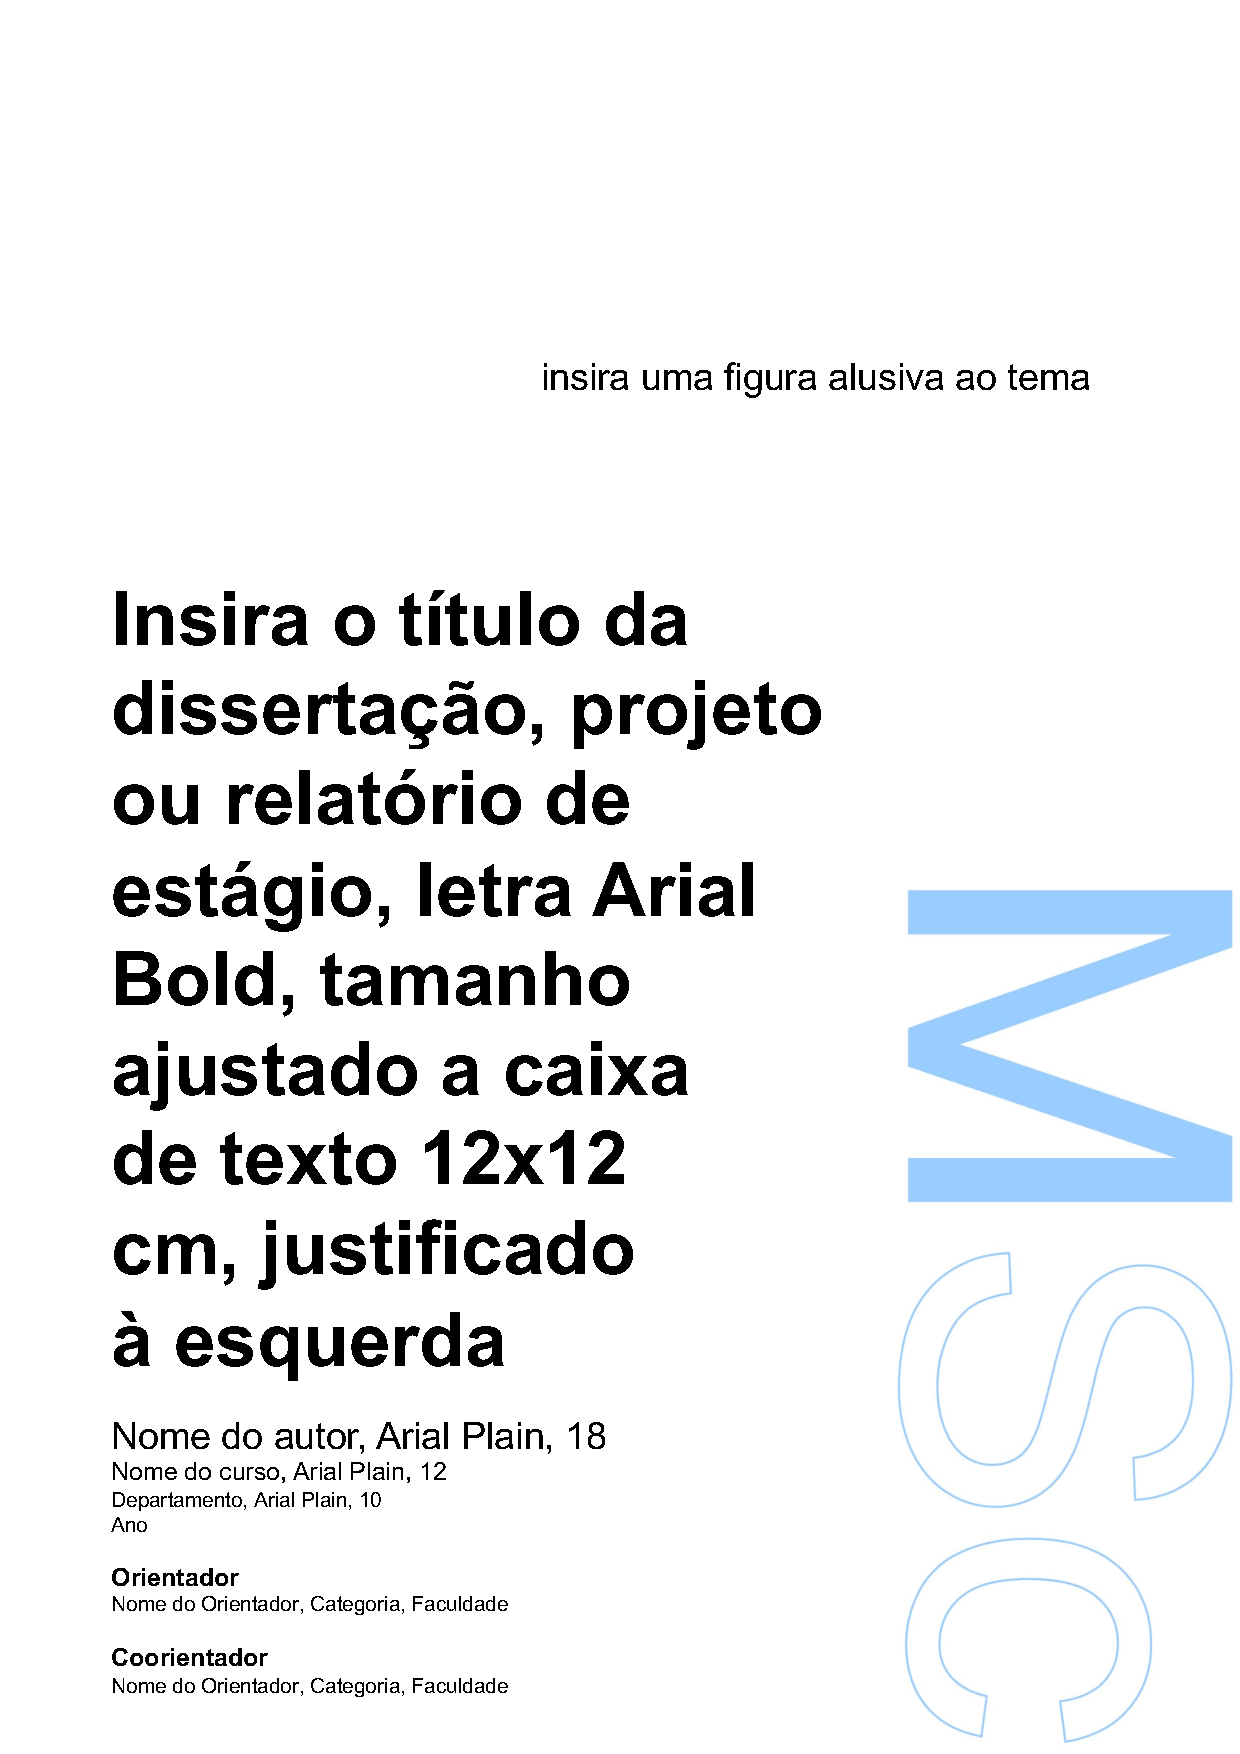
\includepdf[pages=1]{FrontPage-MSc.pdf}
%\cleardoublepage
%\includepdf[pages=2]{FrontPage-MSc.pdf}
%\cleardoublepage

\beforepreface%



% \prefacesection{Abstract}

% A long, long time ago... 

% This section should summarize the content of the dissertation, namely: explain the context of problem, describe the problem itself and address the work done to mitigate/solve the problem. Results and/or contributions should be mentioned.

% \prefacesection{Resumo}
% Há muito, muito tempo

% See the Abstract.
% Test for real
% Test

% \prefacesection{Agradecimentos}

% Obrigado a todos, obrigado \ldots

\prefacesection{Acknowledgements}
First and foremost, I want to thank professors Nelma Moreira and Rogério Reis, who have assisted me this last year. Their help, guidance, willingness and friendliness were fundamental for this work and me.
Thankfulness will never be enough to describe what I feel for my friends and family, who have helped me carry my woes and solaces along this journey. I am especially grateful to my mom and dad for taking care of me.
Lastly, I would also like to thank my work colleagues, who have been very thoughtful and patient with me along the way. 

\prefacesection{Abstract}
%Regular expressions (\emph{regex}) formalize a class of patterns definable over strings, corresponding to the family of regular languages in automata theory. They provide a declarative mechanism for specifying sets of strings, making them central both to theoretical models of computation and to practical applications such as string matching, input validation, and text parsing. Despite their utility, improperly constructed regular expressions can introduce serious security vulnerabilities. One of the most critical threats is the \ac{ReDoS} attack, in which carefully crafted inputs cause the regex engine to perform excessive and redundant processing. This results in dramatic slowdowns or even complete unresponsiveness of the system. \ac{ReDoS} poses a significant risk to web applications, APIs, and other input-facing systems, where user-controlled input is matched against vulnerable patterns.
\noindent Regular expressions (\emph{regex}) formalize a class of patterns definable over strings, corresponding to the family of regular languages in automata theory. They provide a declarative mechanism for specifying sets of strings, making them central both to theoretical models of computation and to practical applications such as string matching, input validation, and text parsing. Despite their utility, certain implementations of regular expression engines (particularly those based on backtracking) can introduce serious security vulnerabilities when combined with specific patterns. One of the most critical threats is the \ac{ReDoS} attack, in which carefully crafted inputs cause the regex engine to perform excessive and redundant processing. This results in dramatic slowdowns or even complete unresponsiveness of the system. \ac{ReDoS} poses a significant risk to web applications, APIs, and other input-facing systems, where user-controlled input is matched against vulnerable patterns.

\noindent In this work, bounded quantifiers (counting) were implemented in \textit{FAdo}. With this, we also propose a system to address \ac{ReDoS} by transforming regular expressions into a modified position automaton, a \ac{NFA} that tracks the exact start and end positions of all matches within an input string. This structure enables a matching function that computes all match positions, including overlapping ones, without relying on backtracking. By exhaustively and efficiently exploring the automaton's transitions, our approach avoids the exponential blowup typical of vulnerable engines, while preserving a somewhat full regex expressiveness.

\noindent We also review existing solutions present in state-of-the-art programming languages and libraries, such as \emph{RE\#} \cite{resharp_tool_paper} and \emph{Hyperscan} \cite{hyperscan_paper}.

\textbf{Keywords:} regular expressions, ReDoS, position automata, nondeterministic finite automata, pattern matching.

\prefacesection{Resumo}
\noindent As expressões regulares (\emph{regex}) formalizam uma classe de padrões definíveis sobre cadeias de caracteres, correspondendo à família das linguagens regulares na teoria dos autómatos. Fornecem um mecanismo declarativo para especificar conjuntos de cadeias, sendo, por isso, centrais tanto para modelos teóricos de computação como para aplicações práticas, tais como procura de padrões, validação de dados e análise de texto. Apesar da sua utilidade, certas implementações de motores de expressões regulares (particularmente aqueles baseados em \textit{backtracking}) podem introduzir vulnerabilidades de segurança graves quando utilizam padrões específicos. Uma das ameaças mais críticas é o ataque \ac{ReDoS}, onde certas entradas levam o motor de regex a realizar processamento excessivo e redundante. Isto resulta em lentidões significativas ou mesmo na completa inoperacionalidade do sistema. O \ac{ReDoS} representa um risco significativo para aplicações web, APIs e outros sistemas voltados para entrada de dados, onde a entrada controlada pelo utilizador é comparada com padrões vulneráveis.

\noindent Neste trabalho, foram implementados quantificadores limitados (contagem) no \textit{FAdo}. Com isto, propomos também um sistema para mitigar o \ac{ReDoS}, ao transformar expressões regulares num autómato de posições modificado --- um \ac{NFA} que regista exatamente as posições de início e fim de todas as ocorrências dentro de uma cadeia de entrada. Esta estrutura permite que uma função de \textit{matching} calcule todas as posições de ocorrência, incluindo as sobrepostas, sem recorrer a \textit{backtracking}. Ao explorar de forma exaustiva e eficiente as transições do autómato, a nossa abordagem evita a explosão exponencial típica de motores vulneráveis, mantendo, ao mesmo tempo, uma expressividade relativamente completa das expressões regulares.

\noindent Analisamos também soluções existentes em linguagens e bibliotecas de programação de ponta, como o \emph{RE\#} \cite{resharp_tool_paper} e o \emph{Hyperscan} \cite{hyperscan_paper}.

\textbf{Palavras-chave:} expressões regulares, ReDoS, autómatos de posições, autómatos finitos não deterministas, correspondência de padrões.

\dedicationpage{Dedico a \ldots}

% end of thesis preamble
\afterpreface%

%% main tex here
%% By putting the chapter names here, one can just comment the content in the chapters 
%% and produce a pdf with the correct chapter number.
%% If you want further configurability you can use subfiles package
%% https://www.ctan.org/pkg/subfiles

%\chapter{Introdução}\label{chap:intro}
\chapter{Introduction}\label{chap:intro}

In this chapter, the problem is overviewed, the study’s importance is explained along with goals for the proposed solution. 

\section{Background}
Despite recent advances in~\cite{cloud}, .....

%\chapter{Background}\label{chap:back}
\chapter{Background}\label{chap:back}

This chapter has the ``Instructions for preparing and writing M.Sc. Dissertations'' (Research-oriented work), 
Version 1.0, January, 7$^{th}$, 2015 from prof. Inês Dutra. It was originally written in English so it was kept as such. It was some additions from Pedro Brandão.

\section{Before Starting}
%%%%%%%%%%%%%%%%%%%%%%%%%%%%%%%%%%%%%%%%
Before starting your dissertation, you need to \textbf{define} what is the subject you are going to work
with and perform a \textbf{thorough systematic} bibliography review of the theme you chose.
What is a systematic review? It is the one where you search the web or books for the subject, and
define rules for filtering papers in two sets “included” and “excluded” and explain why some papers
go to one set or the other.
In order to start the search, you need to prepare keywords related to your subject and prepare
queries to be used in Google Scholar, Scopus, MesH etc. These search engines will return a number
of papers on the subject you are looking for.\textbf{You need to read at least the abstract and 
conclusions of every paper retrieved after your search}. Now, you filter out only the ones you
think are very closely related to your research work, and give a reason for choosing those papers.

\section{Bibliography}
%%%%%%%%%%%%%%%%%%%%%%%%%%%%%%%%%%%%%%%%
 Start organizing your bibliography file. Choose one of the standards available to start organizing
your references. Usually your department/faculty has clear rules about the standard to be used. If
you are formatting your text using \LaTeX, most references found during your bibliographic search
can be exported in BibTeX format.

\subsection{Bibliography Section}
%---------------------------------------
Your dissertation needs to have a Bibliography Section with a list of the cited works you have in
the text. In the process of writing your dissertation, make sure to properly refer the authors you are
basing your text on. For example, “Yaacoub et al.~\cite{yaacoub2012} discovered that\ldots”. In this sentence, Yaacoub is the
first author of one of the publications you list in the Bibliography Section of your dissertation and~\cite{yaacoub2012} is the link that connects this citation to the publication in the bibliographic list. If your
bibliographic entry has only one author, you cite only the author's surname. If the bibliographic
entry has two authors you cite the two authors' surnames (e.g., Clausen and Jacquet~\cite{Clausen2003}). If the
bibliographic entry has more than two authors, you can use the expression “et al.”, like in the
example shown before.

You should avoid as much as possible web site references. Only in some cases, illustration, showing trends, are they acceptable.

References should be used to back up claims made. Specially in the introduction section, sentences that stipulate something should be backed by references that assert that claim (e.g.: \emph{Android, in December 2016, was the most widely used mobile operating system~\cite{netMarketShareMobileOS}\footnote{An example where a web link to a recognized market analysis company would be valid. Note that the time which the report was seen is very relevant.})}

\section{Inserts}
%%%%%%%%%%%%%%%%%%%%%%%%%%%%%%%%%%%%%%%%
Every picture, graph, diagram, algorithm, etc. needs to have a caption and a number, and needs to
be cited and explained in the text. The mere existence of a picture, etc. does not exempt it of a description. 

\subsection{Copyrights and image usage}
%---------------------------------------
If you want to use any picture, graph, diagram, etc. in your
dissertation from one of the publications, you need to make sure that you can use it (check the copyright rules). If the copyright
rules allow you to reproduce the picture (or others) in your text, you need to insert a reference to the
source (where the picture was taken from) in the caption. If you are allowed to use a picture, but
want to slightly modify it, you need to say in the caption: Adapted from [1] (where [1] is the
number of your reference in the Bibliographic Section).


\section{Chapters/Organization}
%%%%%%%%%%%%%%%%%%%%%%%%%%%%%%%%%%%%%%%%
\begin{description}
   \item[Chapter 1: Introduction:]
This should be a summary of what comes in the next chapters. Here you explain in two to five
pages: 
\begin{inparaenum}[(1)]
   \item the context of your work highlighting and defining the problem you need to solve,
   \item what you want to do (objectives),
   \item why you want to do it (motivation),
   \item how you want to achieve your objectives (methodology), always supporting your text on the available literature,
   \item contributions (results that confirm that you achieved your objectives),
   \item organization of the chapters that come next.
\end{inparaenum}

\item[Chapter 2: Basic Concepts:]
In this chapter you need to present the foundations of your work: theoretical aspects, background
material, etc. All that is needed to understand the terminology and expressions used in the remaining
chapters.
\item[Chapter 3: Related Work:]
Here you need to discuss about other works in the literature that do something similar to what
you want to do. You need to cite and discuss the relevant papers you chose to include in your study
during your survey. Explain what others do, why it is not sufficient, and why you need to do what
you want to do. It is helpful to define some criteria to compare your work against others, and
build a table with main characteristics of other works contrasting to what you want to do. In other
words, in which aspects is your work different from others?
\item[Chapter 4: Your Work:] this chapter describes the contributions of the work done. If it is based on prior work (continuation of the project or using prior developed work), it should only describe what is the new work done. If references are needed, it should be clear what is the prior work and what is the new contribution.
\item[Chapter 5: Materials and Methods:] should have:
   \begin{itemize}
      \item Definition of Experiments (if any)
      \item Definition of Evaluation Metrics
   \end{itemize}
\item[Chapter 6: Results and Analysis]
\item[Chapter 7: Conclusions and Future work:] 
         this should restate the problem and iterate through the solution(s) analyzing the advantages and contributions. The limitations and unsolved problems should also be described.
         It should also describe the potentiality of new research/development that the work enables, the future work.
   \begin{itemize}
      \item Research Summary
      \item Main Findings
      \item Limitations
      \item Future Work
      \item Conclusion
   \end{itemize}
\end{description}
During writing, some of these chapters may collapse into just one.\textbf{Your work (chapters 4-7) should account for at least 50\% of your whole dissertation.}

\subsection{Contents of each chapter}
%---------------------------------------
You should start each chapter with a summary of its objective and contents, preferably relating to previous ones. At the end of the chapter provide a conclusion/summary of it, preferably connecting it to the next one.

%vim: set fo+=aw tw=80 spl=en_gb spell: syntax spell toplevel  :


%\chapter{Estado da Arte}\label{chap:stat}
\chapter{Estado da Arte}\label{chap:stat}

Sem conteúdo relevante, apenas com texto para ocupar o espaço.

\section{Section example}
\lipsum[1-6]
\section{Second Section example}
\subsection{SubSection example}
\lipsum[7-10]



%\chapter{Desenho da Arquitetura}\label{chap:syst}

\chapter{Implementation}\label{chap:devel}

The implementation chapter gives insights into 

\section{Client-Server Architecture}

This section describes the client-server architecture, which is important in the development of the application. It focuses on coordination of the mobile/web clients developed using Flutter and the Firebase server to support instant data flow, secure sign-in, and retrieval/storing of the data.

\begin{lstlisting}[
  %language=yaml,                   % Specify language for syntax highlighting
  numbers=left,                    % Add line numbers on the left
  numberstyle=\tiny\color{gray},   % Style line numbers (smaller, gray)
  basicstyle=\footnotesize,         % Set code font size (smaller)
  caption=Flutter Project Dependencies,        % Add a caption
  frame=single,                    % Add a single frame around the listing
  showtabs=false,                   % Hide tabs (optional)
  breaklines=true,                   % Allow line breaks (optional)
  breakatwhitespace=false           % Prevent breaks within words (optional)
]
dependencies:
  flutter:
    sdk: flutter
  firebase_core: latest_version
  firebase_auth: latest_version
  cloud_firestore: latest_version
\end{lstlisting}


%\chapter{Desenvolvimento}\label{chap:dese}
\chapter{Experiências e Testes}\label{chap:tests}

O referente ao ``Materials and Methods'' do capítulo~\ref{chap:back}.

Outro acrónimo pode ser \ac{TCP} (que deve estar expandido aqui, apesar de ter sido usado já no capítulo \ref{chap:devel}).

\lipsum
 

%\chapter{Resultados e análise}\label{chap:results}
% !TEX root = thesis.tex

\chapter{Results and Discussion}\label{chap:results}

This is a test

\section{Evaluation}

The methods of evaluating
 

%\chapter{Conclusões}\label{chap:conc}
\chapter{Conclusões}\label{chap:conc}

\lipsum[4-6]

\section{Trabalho Futuro}\label{sec:trab}

\lipsum[1-3]



%% appendix
\appendix
%% \include{app1}

%% references
%\renewcommand{\bibname}{Referências} % o babel portuguese coloca Bibliografia
% os meses do ficheiro bib poderão aparecer em inglês, caso se pretenda deve-se colocar o texto em português explicitamente no ficheiro bid
\cleardoublepage%
\phantomsection%
\addcontentsline{toc}{chapter}{\bibname}
\bibliographystyle{plainnaturlAuthor} % use plainnaturlAppear to order references by appearance 
% usually it is by author on thesis, to ease Author lookup
%\nocite{*}  % Include all entries in references.bib, not just the ones cited.
\bibliography{refs} %changed the env to make it a numbered chapter

%% bye
\end{document}
